% Intended LaTeX compiler: pdflatex
\documentclass[11pt]{article}
\usepackage[utf8]{inputenc}
\usepackage[T1]{fontenc}
\usepackage{graphicx}
\usepackage{longtable}
\usepackage{wrapfig}
\usepackage{rotating}
\usepackage[normalem]{ulem}
\usepackage{amsmath}
\usepackage{amssymb}
\usepackage{capt-of}
\usepackage{hyperref}
\usepackage[final]{latex/acl}
\usepackage{times}
\usepackage{latexsym}
\usepackage[utf8]{inputenc}
\usepackage{microtype}
\usepackage{inconsolata}
\usepackage{enumitem}
\usepackage{multirow}
\setcounter{secnumdepth}{1}
\date{\today}

% If the title and author information does not fit in the area allocated, uncomment the following
%
%\setlength\titlebox{<dim>}
%
% and set <dim> to something 5cm or larger.
% Author information can be set in various styles:
% For several authors from the same institution:
% \author{Author 1 \and ... \and Author n \\
%         Address line \\ ... \\ Address line}
% if the names do not fit well on one line use
%         Author 1 \\ {\bf Author 2} \\ ... \\ {\bf Author n} \\
% For authors from different institutions:
% \author{Author 1 \\ Address line \\  ... \\ Address line
%         \And  ... \And
%         Author n \\ Address line \\ ... \\ Address line}
% To start a separate ``row'' of authors use \AND, as in
% \author{Author 1 \\ Address line \\  ... \\ Address line
%         \AND
%         Author 2 \\ Address line \\ ... \\ Address line \And
%         Author 3 \\ Address line \\ ... \\ Address line}

\author{
Debarghya Datta \and Soumajit Pramanik \\
Department of Computer Science\\
Indian Institute of Technology, Bhilai\\
\texttt{\{debarghyad,soumajit\}@iitbhilai.ac.in}\\
}

\newcommand{\td}[1]{\textcolor{blue}{[{SP: #1}]}}
\newcommand{\ts}[1]{\textcolor{blue}{[{DD: #1}]}}

\title{Unsupervised Named Entity Disambiguation for Low Resource Domains}
\begin{document}
\maketitle
\begin{abstract}
In the ever-evolving landscape of natural language processing and
information retrieval, the need for robust and domain-specific entity
linking algorithms has become increasingly apparent. It is crucial in
a considerable number of fields such as humanities, technical writing and
biomedical sciences to enrich texts with semantics and discover more
knowledge. The use of Named Entity Disambiguation (NED) in such domains requires handling noisy
texts, low resource settings and domain-specific KBs.  Existing
approaches are mostly inappropriate for such scenarios, as they either depend on
training data or are not flexible enough to work with domain-specific KBs. Thus in this work, we present an unsupervised approach leveraging
the concept of Group Steiner Trees (GST), which can identify the most relevant candidates for entity disambiguation using the
contextual similarities across candidate entities for all the mentions present in a document. We outperform the state-of-the-art unsupervised methods by more than 40\% (in avg.) in terms of Precision@1 across various domain-specific datasets.

\end{abstract}
% Add it to abstract if required
%We evaluate our ranking approach in a both Supervised (small training data) and Unsupervised (no training data) setting to mimic the real-life use-case of our algorithm.
% Our open-sourced data and code is available \url{https://github.com/deba-iitbh/GST-NED} repo.

% \keywords{Named Entity Recognition, Group Steiner Tree, Entity Linking, Domain-specific, Low-resource}

\section{Introduction}
Named Entity Disambiguation (NED) is the task of resolving the ambiguity associated
with entity mentions in a document by linking them to the appropriate entries in a
Knowledge Base (KB).
% (see example in Fig. \ref{fig:el-task1}).
% Traditionally hand-designed features \cite{cucerzan2007large, kulkarni2009collective} have been proposed to perform NED by calculating similarities between the mentions and their corresponding candidates; however, recently neural-network based
% methods~\cite{kolitsas-etal-2018-end,gillick-etal-2019-learning,li-etal-2020-efficient,decao2021autoregressive}
% that embed the mention context and candidate description in the same vector space are found to offer the state-of-the-art solutions, but are often developed and evaluated on generic Knowledge Bases(eg. Wikidata, DBpedia) and large datasets that are not readily available for domain-specific tasks.
% In recent years, NED has found its application in diverse domains such as digital humanities, art and architecture, literature and biomedical science for searching~\cite{meij2014entity}, question answering ~\cite{yih-etal-2015-semantic} and information extraction~\cite{nooralahzadeh-ovrelid-2018-sirius} tasks.
Recently, NED has been applied in various fields, including digital humanities, art, architecture, literature, and biomedical science, for tasks such as searching~\cite{meij2014entity}, question answering
~\cite{yih-etal-2015-semantic} and information
extraction~\cite{nooralahzadeh-ovrelid-2018-sirius}.

The key challenges in such domain specific NED tasks are twofold - 
(a) they provide little or no training data with ground truth annotations and 
(b) the associated knowledge graphs (KG) are typically small and with no or very limited entity descriptions~\cite{shi2023knowledge}. In order to deal with such challenges, in this work we consider the setting where entity disambiguation is needed to be performed with \emph{absolute absence of annotated data}.
%where neither the candidate generator nor the disambiguation technique (the two key modules of any typical entity linker) can leverage any annotated data.
In such constrained scenarios, leveraging the state-of-the-art neural entity linkers become infeasible as they are primarily dependent on a 
large corpus of annotated data and long enough entity descriptions from KG~\cite{CadavidSnchez2023EvaluatingEE, arora2021low}.
Similarly this setting also disqualifies unsupervised NED approaches such as ~\cite{pan2015unsupervised} which rely on labeled data to generate candidate entities such as domain-adaptive transformer-based models~\cite{aydin-etal-2022-find}, BLINK~\cite{wu2019zero}, Zeshel~\cite{logeswaran-etal-2019-zero}, and auto-regressive models like GENRE~\cite{decao2021autoregressive}.
% \td{Add references to BLINK, autoreregressive models, zeroshot models}


%As they are applied in resource-constrained environments, with little or no training data and human-curated small KB with small entity descriptions, the training of state-of-the-art (SOTA) EL solutions becomes unfeasible as they heavily rely on sentence embeddings for semantic similarity. The inadequacy of detailed entity descriptions hinders the effective application of such solutions within the context of these KBs.
% Moreover, companies may have their proprietary KGs where some entities are only meaningful with respect to the company. In all these cases, available labeled data cannot generalize to the corresponding specialized KGs.

% In literature, only a few approaches exist which qualify for the constrained setting we consider - most of them are graph based approaches relying on distances between the mentions~\cite{hoffart2011robust}, PageRank/random walk~\cite{guo2018robust} and Graph Ranking~\cite{alhelbawy2014graph}.  
% Subsequently, in \cite{arora2021low} the authors proposed a singular value decomposition based approach where they show that the gold entities tend to lie in a low-rank subspace of the full entity embedding space. 
% However, all these approaches are typically limited by their capability of correctly linking the entities.

% \begin{figure}
% \centering
% \includegraphics[width=\linewidth]{./pix/el-task2.eps}
% \caption{Example of Entity Linking with underlined mentions and corresponding list of candidates. The correct candidate for each mention is highlighted in red.}
% \label{fig:el-task1}
% \end{figure}

In the literature, only a few approaches fit our constrained setting such as graph-based using mention distances~\cite{hoffart2011robust}, PageRank/random walk based~\cite{guo2018robust}, and graph ranking based~\cite{alhelbawy2014graph}. A recent approach by~\cite{arora2021low} also explores singular value decomposition, showing gold entities in a low-rank subspace. However, these methods often struggle in achieving the required efficacy while disambiguating entities.

%Although being the state-of-the-art in the considered setting, the key limitation of this approach is that it cannot perform EL for KG entities that are not observed during computation of entity embeddings. 


In this work, we present a novel unsupervised NED approach for domain specific low-resource 
scenarios, which leverages the concept of Group Steiner Trees (GSTs) ~\cite{garg2000polylogarithmic}.
In this approach, we map the candidate entities for each mention in the document, to nodes in the associated knowledge graph, obtain the subgraph connecting these nodes and then extract minimum cost GSTs from this sub-graph. Such GSTs facilitate collective entity disambiguation exploiting the
fact that the entities that are truly mentioned in
a document (the `gold entities') tend to form a
dense subgraph among the set of all candidate entities in the document.

%based on the inherent contextual proximity among the aforementioned entity candidates. 
%Within the document context, mentions inherently pertain to specific contexts, underscoring the necessity for collective disambiguation to influence the associated candidates collectively. Motivated by this insight,  we extract an induced subgraph comprising mention candidates for various mentions within the document. Our objective is to pinpoint a minimum-cost Group Steiner Tree (GST) within this subgraph, with the anticipation that its terminal nodes will correspond to disambiguated candidates. 

\begin{figure*}
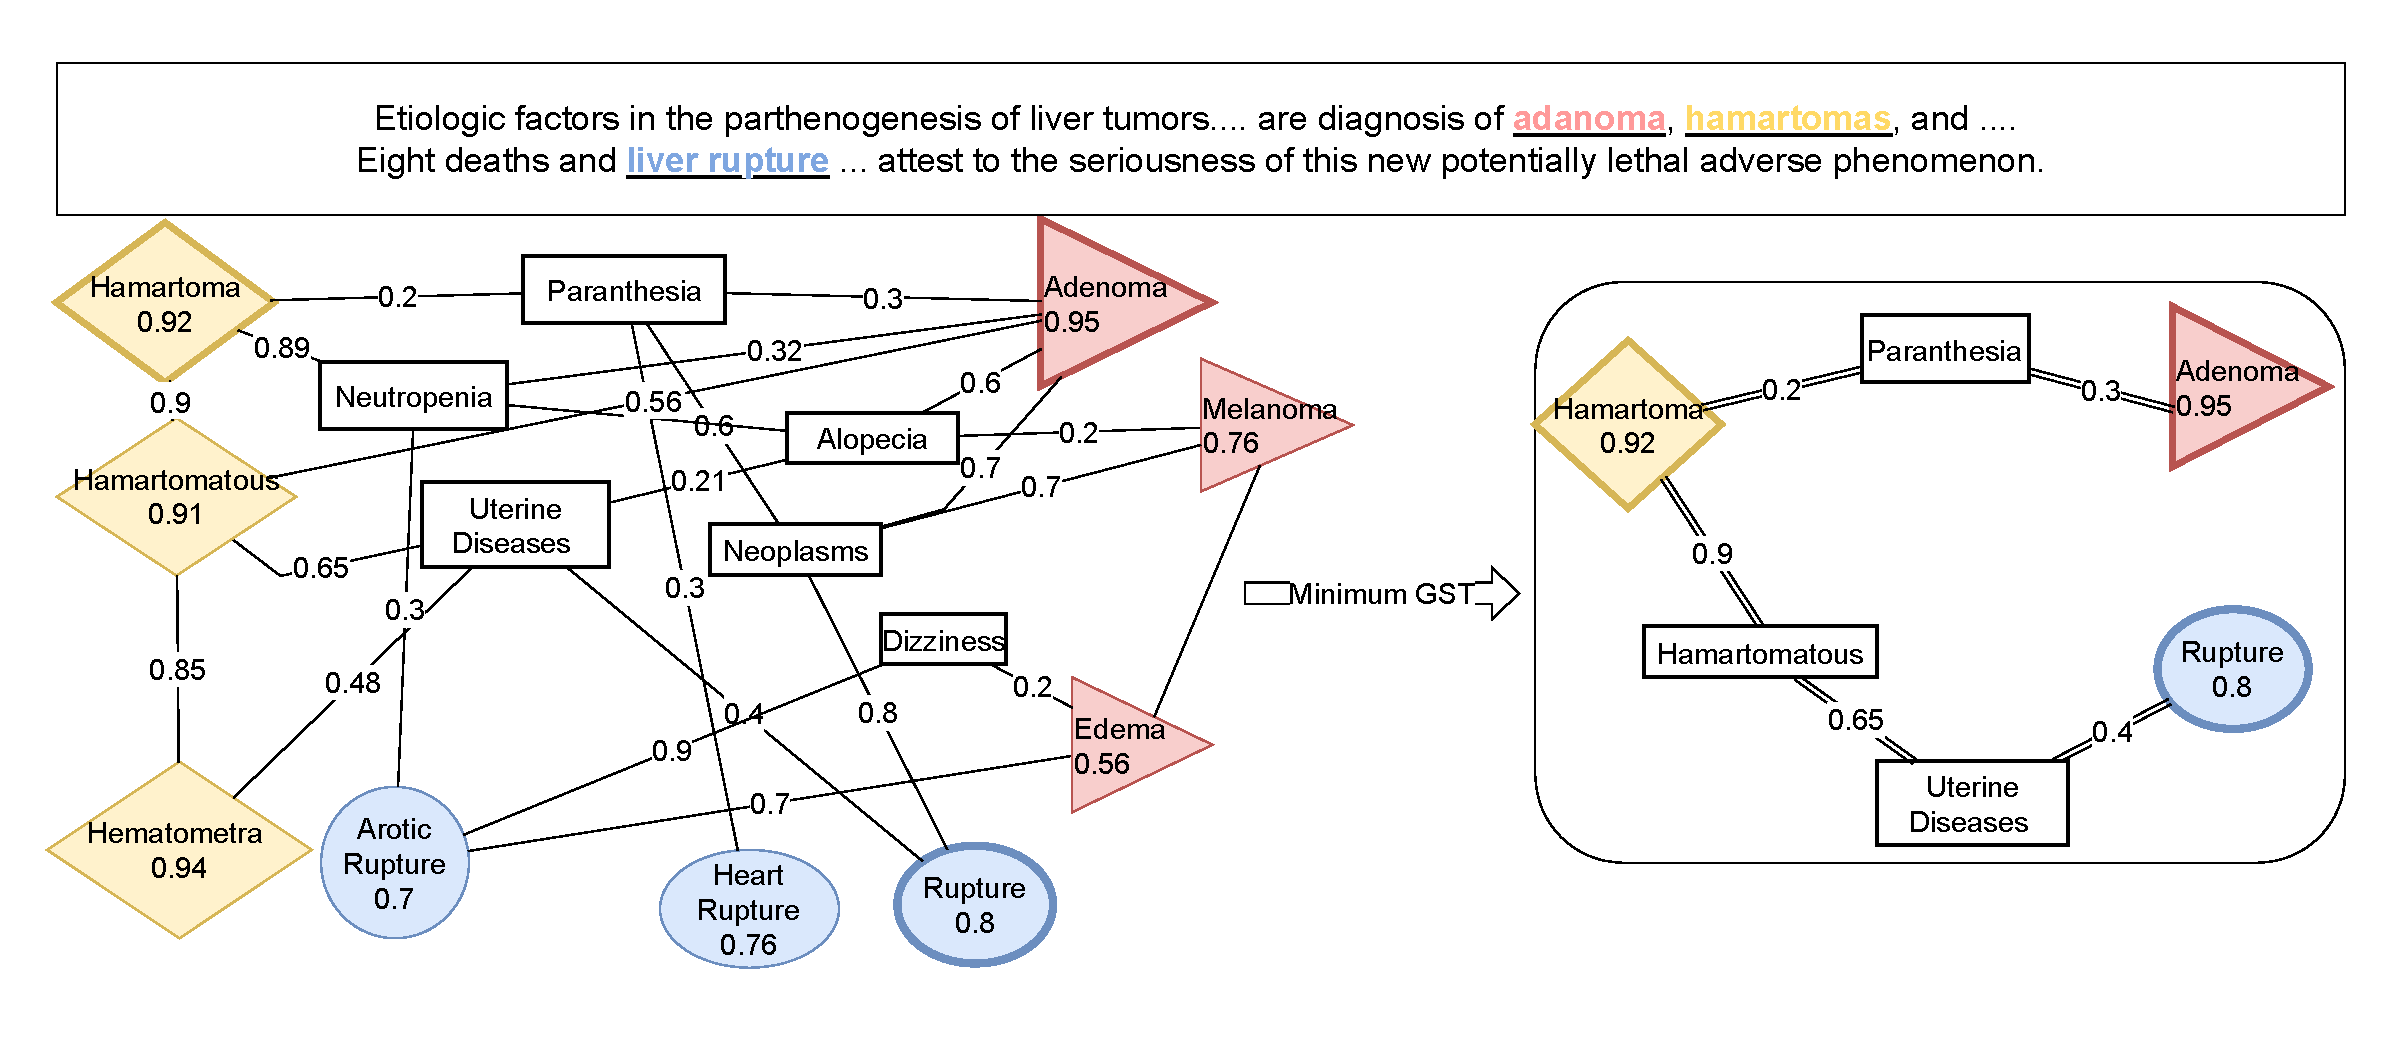
\includegraphics[width=\linewidth]{./pix/pipeline_m4.pdf}
%\caption{Extraction of subgraph from the KB with all the candidates. The candidates for "adenoma" are in red, "hamartomas" are in yellow and candidate for "liver rupture" is in blue. The induced subgraph is shown at the left and the minimum cost GST is shown using the box at the right.}
\caption{Proposed GST-NED approach: The sample document at the top contains three mentions; the subgraph extracted from the KB is shown at the left and the minimum cost GST is shown using the box at the right. In the induced subgraph, the candidates for `adenoma' are marked in red, `hamartomas' are marked in yellow and `liver rupture' are marked in blue.}
\label{fig:el-task}
\end{figure*}


%The approach also provides promising results when combined with supervised approaches.
In summary, our main contributions are the following -
%\begin{itemize}
 %   \item 
(a) We propose an unsupervised \textbf{G}roup \textbf{S}teiner \textbf{T}ree based \textbf{N}amed \textbf{E}ntity \textbf{D}isambiguation (\emph{GST-NED}) method which is capable to perform NED for low resource domains at the absence of any annotated data;
(b) We compare our proposed approach with several state-of-the-art baselines across multiple domain specific datasets and demonstrate its superior performance
%Our proposed approach outperforms the existing unsupervised methods,
with significant improvements in the metrics (more than $40\%$ in avg. in Precision@1 scores)~\footnote{Code is available at \url{https://github.com/deba-iitbh/GST-NED}}. 

    %\item Our proposed method (GroSTEL) is also showed to improve the performance of supervised EL models when used in conjunction.
%\end{itemize}


% \section{Related Works}
% \textbf{Open-Domain EL} - TODO
% \noindent
% \textbf{Domain-specific EL} against domain-specific knowledge bases has not
% been studied extensively in the
% literature. AGDISTIS\cite{usbeck2014agdistis} employs a
% knowledge-base-agnostic approach based on the HITS algorithm,
% utilizing gazetteers compiled from resources like Wikipedia for string
% matching in mention detection.  REDEN\cite{brando2016reden}, a graph
% centrality-based approach linking French authors to literary criticism
% texts, necessitating additional linked data aligned with a custom
% knowledge base (DBPedia). Operating within a domain-specific
% low-resource setting, our work faces challenges, including restricted
% access to large corpora for computing popularity priors, absence of
% suitable named entity linking tools and gazetteers, and insufficient
% labeled training data, making the application of state-of-the-art
% systems challenging.



% In this section, we present our problem statement in detail and then delineate the different components of our proposed method. 

\section{Problem Statement}
%We first formalize the task of interest. 
% Let $d$ be a single document from a collection $D$ of documents.
Similar to most previous works in the NED literature (with a few exceptions \cite{kolitsas2018end, sil2013re}), we assume that document-wise mention spans
(usually obtained by a named entity recognizer) are already
provided.
Let $d$ be a single document from a collection $D$ of documents.
Also, let $M_d = \{m_1, m_2, \ldots , m_M\}$
be the set of $M$ mentions contained in $d$, and let $\mathcal{E}$
be the collection of all the entities contained in the reference domain specific Knowledge Graph $KG$. The task here is to find, for each mention $m_i$ the correct entity $e \in \mathcal{E}$ it refers to.

Typically, given the set of mentions, an NED approach performs the disambiguation in two steps - 
%(a) Mention detection, where text spans (denoted as mentions) which can be potentially mapped with KG nodes, are extracted from text~\footnote{the sentence or passage/document from which mention is extracted is denoted as its context}, (b
(a) Candidate generation, where candidate entities from the $KG$ are retrieved for each of the mentions, and (b) Candidate Ranking, where the candidate entities are ranked based on their propensities to be mapped with the corresponding mentions. 
Our primary focus in this study is the candidate ranking/disambiguation step. 
%In this context, we define the text span containing an entity as the mention, and the sentence in which the mention is embedded as the mention's context. Each candidate sourced from the knowledge base is presumed to possess a label and may optionally have a corresponding description.
In the following, we describe our proposed candidate ranking method and mention the approaches adhered for the other step.
%\subsection{Mention Detection}
%Recognizing the crucial role of this step in ensuring robust linking and accuracy, we opt for the Gold NER approach, given its independence from the linking process, as mention-detection is out of this work's scope. Though, off-the-shelf state-of-the-art (SOTA) Named Entity Recognition (NER) solutions can be used with the conjunction of a rule-based NER model tailored to the heuristics of a particular domain.

\section{Methodology}
\subsection{Candidate Generation}
We index the domain specific $KG$ and use fuzzy text search \cite{max_bachmann_2021_5584996} to retrieve candidates based on the surface form of the annotated mention. This is found to be the standard practice in most of the recent unsupervised NED approaches~\cite{yang2023b, simos2022computationally}
%Most of the candidates in our $KG$ have a set of aliases; so a weighted fuzzy search is employed to help in cases where the mention and the $KG$ label are almost the same but not identical (e.g. Dublin vs. Dublyn). 
Fuzzy text search returns a confidence value with each potential match; we keep only the candidates which are returned with more than $0.75$ confidence value (chosen empirically)~\footnote{In case of exact match with a KG node, we consider it to be the correct match for the mention and skip the candidate ranking step.}.

\subsection{Candidate Ranking}
% \textbf{Subgraph Extraction:} We leverage the $KG$ to extract an induced
% subgraph of all the entity candidates 
% obtained through the candidate generation step. In order to ensure a manageable graph size, we restrict ourselves to adding paths of maximum three hop distance between any pair of entity candidates.
% To further enhance
% the extracted graph, we add node and edge weights to the graph. For node weight, we use the Jaro
% winkler distance \cite{wang2017efficient} that assigns weights to the graph's entities based
% on their similarities with the corresponding mentions. In order to assign the edge-weights, we obtain the structural embeddings of the nodes in the $KG$ using Node2Vec \cite{grover2016node2vec} and compute the cosine similarities of the embedding corresponding to each pair of nodes connected in the induced graph.
% In Fig.~\ref{fig:el-task}, we demonstrate a document with three mentions and the corresponding induced subgraph of the candidate entities.

We use the knowledge graph ($KG$) to create a subgraph connecting all pairs of candidate entities obtained from the candidate generation step for a particular document $d$. To keep the graph size manageable, we limit path lengths to be a maximum of three hops between entity candidates. We further enhance the graph by adding node weights based on the Jaro-Winkler distance~\cite{wang2017efficient} (reflecting similarities of candidates with mentions), and edge weights based on cosine similarities of Node2Vec \cite{grover2016node2vec} structural embeddings of the endpoints. 
In Figure~\ref{fig:el-task}, we depict a document with three mentions and the corresponding induced subgraph of candidate entities (left side).


\noindent
\textbf{Finding GST:} Our approach to identify the correct candidates
relies on the intuition that a gold entity candidate from a document $d$ should be more tightly connected with other gold candidates in the induced subgraph   
compared to other non-gold candidates.
In other words, we expect the gold entities within the induced subgraph to form cohesive and closely linked subgraphs due to their contextual proximities (as they are used in the same document).
%\noindent
%\td{First define Terminals in our context.}
In order to exploit this intuition, we first define the notion of terminals - for every mention $m_i$, we denote the corresponding candidate entity nodes as the terminal nodes for that mention and group them together as $T_i$. 
%In other words, all the candidate entity nodes for the ${i}^{th}$ mention, would be grouped under the terminal group $T_i$. 
Further the task remains is to select the correct candidate node from each terminal group for which we leverage the concept of Group Steiner Trees (GST)~\cite{ding2006finding,pramanik2024uniqorn} as defined below,
\begin{itemize}[topsep=2pt,itemsep=0pt,partopsep=0pt, parsep=0pt]
\item Given an undirected and weighted graph \((V, E)\) and given groups of terminal nodes \(\{T_1, . . . ,T_l\}\) with each \(T_\nu \subseteq V\), compute the minimum-cost tree \((V^*, E^*)\) that connects at least one node from each of \(\{T_1, . . . ,T_l\}\): \(\min \sum_{ij \in E^*} c_{ij}\) s.t. \(T_\nu \cap V^* \ne \emptyset, \ \forall T_\nu\).
\end{itemize}
In our case, we consider $c_{ij}=(1 - w_{ij})$ where $w_{ij}$ represents the edge weight between nodes $i$ and $j$. 
%and each terminal group $T_v$ consists of all the entity candidates for a particular mention
% for all the edges and each terminal group $T_v$ to be consisting of all the entity candidates for a particular mention.
As per definition, each GST would have to necessarily choose at least one candidate entity from each of the terminal groups. Hence, each detected GST would provide at least one potential solution to the entity disambiguation problem. 
%\td{DROP NEXT LINE, Can we not highlight the `at least one' part.}
%Hence, it is sufficient if the returned GST contains one candidate entity from the group of each mention. 
As we further posit that the gold candidate entities are more tightly connected compared to non-gold candidates, the probability of the gold candidates to be chosen in the minimum cost GST increases (as the minimum cost GST ensures shorter distances between the chosen candidates and higher weighted edges i.e. lower edge-costs). For instance, in the right side of the Fig.~\ref{fig:el-task}, we depict that the minimum cost GST extracted from the induced subgraph contains all the gold candidate entities corresponding to the mentions in the document. 


\noindent
\textbf{Relaxation to GST-k and Ranking Criteria}: 
In our setting, we actually look for the entity candidates extracted from k least cost GSTs (used k=10 for our work empirically) rather than relying upon only the minimum cost GST. This is for enhancing the robustness of the approach as it allows us to rank the different candidate entities efficiently.
%For feature extraction across all candidates, we leverage the top-k (\(\le\)50) Group Steiner Trees (GSTs) to ensure obtaining features for all candidates. 
%The ranking of terminals/candidates is determined by their presence in multiple GSTs. However, we also take into account other features to further refine their ranking.
We utilize the following three intutive ranking schemes to rank the candidate entities for each mention and choose the higher ranked one -  \textbf{(a) GST count}: Number of GSTs where the candidate is present; the higher the better, \textbf{(b) GST Cost}: Total cost of the GSTs where the candidate is present; the lower the better, and
\textbf{(c) Node Weight:} The sum of node weights in the GSTs where the candidate is present; the higher the better. Subsequently, we compare the performance of all three schemes to choose the best one.
    %\item \textbf{GST Dist}: Total distances of candidate to the other candidates in the GST, the lower the better.

    %\item \textbf{GST Wt Dist}: A weighted version of candidate distances, when edge weights are available, the lower the better.
%\end{enumerate}
\noindent
\textbf{Complexity:} Steiner trees are among the classical NP-complete problems~\cite{ding2006finding}, and this holds for the GST problem too. However, the problem has tractable fixed-parameter complexity when the number of terminals is treated as a constant \cite{downey2013fundamentals}, and there are also good polynomial-time approximation algorithms extensively applied in the area of keyword search over databases \cite{ding2006finding,kacholia2005bidirectional,li2016efficient}. In
\emph{GST-NED}, we build on the exact solution method by \cite{ding2006finding}, which uses a dynamic programming approach and has exponential runtime in the number of mentions (which is typically limited) but has $O(n\log n)$ complexity in the graph size.

\section{Experimental Setup}
% There are very few domain-specific corpora at our disposal for
% conducting EL in domain-specific setting, even though they have been
% widely used in both academic and industrial applications.

\subsection{Datasets}
In order to show the efficacy of our model, we choose the following four datasets from diverse domains of literature, law, museum artifacts and chemicals (see Table.~\ref{tab:data-stat} for more details). 
%The details of the datasets are described below.

\noindent
\textbf{WWO}\footnote{\url{https://www.wwp.northeastern.edu/wwo}} is a collection of textual documents (poems, plays and novels) by pre-Victorian women writers, partially
annotated~\cite{flanders2010encoding} with person, works and places entities. 
%against a personography KB. 
%Due to the pre-victorian English, this dataset becomes challenging for off-the-shelve EL tools, and moreover, there is a lack of standard orthography, lot of spelling variations and ciphered names to call a person.

\begin{table}
\resizebox{\columnwidth}{!}{
\begin{tabular}{lrrrrrr}
Dataset & \#D & \#M & \#N & \#E & \#C & \#R\\[0pt]
\hline
WWO & 76 & 14651 & 9065 & 4936 & 10 & 0.83\\[0pt]
1641 & 16 & 480 & 3503 & 338 & 10 & 0.26\\[0pt]
Artifact & 168 & 6311 & 41180 & 42634 & 11 & 0.66\\[0pt]
%Medic & 135 & 12735 & 13302 & 30592 & 12\\[0pt]
Chemical & 135 & 15769 & 176415 & 249275 & 10 & 0.73\\[0pt]
\end{tabular}
}
\caption{\label{tab:data-stat}Data statistics of the four used datasets: Total number of Documents ($\#D$), Total number of mentions ($\#M$), Number of Nodes ($\#N$) and Edges ($\#E$) in KG, Average number of candidates per mention ($\#C$) and Recall of the candidate entities i.e fraction of mentions with gold entities present among the candidates ($\#R$)}.
\end{table}
%\td{Mention Recall of candidates dataset wise, Mento=ion system config and runtimes.}

\noindent
\textbf{1641}\footnote{\url{http://1641.tcd.ie/}} consists of legal texts in the form of court witness statements recorded after the Irish Rebellion of 1641, partially
%Some of the documents has been annotated~\cite{munnelly2018constructing} with
annotated with person names against a subset of DBpedia KB~\cite{klie2020zero}. 
%Similar to \textbf{WWO}, here also the same linking challenges occur due to old language from the $17^{th}$ century and non-standard orthography.

\noindent
\textbf{Chemical} dataset %\cite{ruas2020linking}
is sourced from the BC5CDR corpus ~\cite{li2016biocreative}. It features a comprehensive human annotations of chemicals, each tagged with unique MeSH identifiers. 
%\td{May skip the next line if not important}
For the categorization of chemicals, the Chemicals vocabulary is sourced from the Comparative Toxicogenomics Database (CTD)~\footnote{\url{https://www.ctdbase.org/}}. 

\noindent
\textbf{Artifact}~\cite{CadavidSnchez2023EvaluatingEE} is a collection of digital descriptions of Museum objects 
%sourced from six online museum collections. Part of the objects were manually 
annotated with four different text fields:
title, detailed description, free-form metadata against the Getty
Arts, and Architecture Thesaurus~\footnote{\url{https://www.getty.edu/research/tools/vocabularies/aat/about.html}}(AAT). 
%The dataset's complexity poses a challenge for Entity Linking (EL) due to the nuanced meanings and substantial text diversity


%To augment the hierarchical structures of these vocabularies, entity relations provided within the BC5CDR dataset are utilized.

%In our endeavor to align diseases with a standardized ontology, we employed the MEDIC Disease vocabulary derived from the Comparative Toxicogenomics Database (CTD)\footnote{\url{https://www.ctdbase.org/}}
%. Simultaneously,

%Further details of the datasets are provided in Table.~\ref{tab:data-stat}. High values of the $\#C$ column indicates the difficulty levels of the NED tasks to be performed on this datasets.

\subsection{Baselines}
To compare the performance of our proposed approach, we leverage the following baselines~\footnote{All the Datasets and Baseline codes are available under MIT \& Apache License.}.
%we evaluate EL performance with the Gold NER entities. Then, supervised ranking performance is evaluated on the curated dataset similarly to state-ofthe-art EL benchmarks. 

\noindent
\textbf{NameMatch}\cite{klie2020zero}. We employ a string-matching approach to select candidates that exactly match the surface form of the mention.

\noindent
\textbf{BLINK*}~\cite{wu2019zero}. We adapt a fine-tuned BLINK model in our domain specific setup for predicting named entities for each mention. As it matches entities to Wikipedia\footnote{\url{https://www.wikipedia.org/}} by default, we subsequently perform a fuzzy matching process to align the predicted entities with our domain specific knowledge base.

% \noindent
% \textbf{String Matching}
% we employed a string-matching approach that selects the most probable
% candidate based on Levenshtein distance. Based on the distance it predicts multiple entities.
% \noindent

\noindent
\textbf{WalkingNED}~\cite{guo2018robust} is a graph-based approach to disambiguate the mention candidates, based on local similarity (surface form similarity) and global similarity (similarity between the semantic signatures of the candidate and the document computed using PageRank). 
%The semantic signature of the candidate and the document is computed using a pagerank algorithm over the induced subgraph extracted from the KG with all the candidates of different mentions in the document. More details on their implementation can be found in their paper.

% \textbf{Zero-to-Hero}
% \cite{klie2020zero} represented the candidate mapping as supervised
% learning-to-rank(L2R) problem, where given a mention and a list of
% candidates, sort the candidates so that the most relevant candidate is
% at the top. They used a set of generic handcrafted features which are
% described in Table \ref{tab:z2h-gst}. SOTA L2R models like gradient boosted
% trees variant LightGBM\cite{ke2017lightgbm},
% RankSVM\cite{joachims2002optimizing} and
% RankNet\cite{burges2005learning} were chosen as they can work with
% low data and allow introspection. They also leverage pretrained
% Sentence-BERT embeddings\cite{reimers2019sentence} trained on Natural
% Language Inference data written in simple English.

\noindent
\textbf{Eigenthemes}~\cite{arora2021low} 
%offers a novel, efficient, and scalable approach to entity linking without requiring supervised training data. It 
is an approach which
leverages the inherent property of `gold entities' to cluster together within the embedding space by representing entities as vectors and utilizing Singular Value Decomposition (SVD).
%, Eigenthemes identifies a low-rank subspace encompassing these relevant entities and their candidates. Candidate entities are then scored based on their proximity to this subspace, guiding the disambiguation process.



\begin{table}[htbp]
\centering
\begin{tabular}{p{2cm}p{2cm}p{1cm}p{1cm}}
Dataset & Model & P@1 & HIT@5\\[0pt]
\hline
 WWO
 & NameMatch	& 0.35 & 0.35 \\
 %& String Matcher & 0.56 & 0.74 \\
 %& DegreeMatch & 0.10 & 0.43 \\
 & BLINK* & 0.07 & 0.09 \\
 & WalkingNED & 0.18 & 0.49\\
 & EigenThemes & 0.14 & 0.45\\
 & GST-NED & \textbf{0.57} & \textbf{0.72}\\
\hline
 1641
 & NameMatch & 0.06 & 0.06 \\
 %& String Matcher & 0.21 & 0.24 \\
 %& DegreeMatch & 0.23 & 0.26 \\
 & BLINK* & 0.05	& 0.11 \\
 & WalkingNED & 0.11 & 0.17\\
 & EigenThemes & 0.17 & \textbf{0.25}\\
 & GST-NED & \textbf{0.20} & 0.22 \\
\hline
Artifact
 & NameMatch & 0.23 & 0.23 \\
 %& String Matcher & 0.46 & 0.61 \\
 %& DegreeMatch & 0.19 & 0.49 \\
 & BLINK* & 0.02	& 0.03 \\
 & WalkingNED & 0.26 & 0.56\\
 & EigenThemes & 0.15 & 0.44\\
 & GST-NED & \textbf{0.54} & \textbf{0.61} \\
\hline
%Medic
 %& NameMatch & 0.03 & 0.03 \\
 %& String Matcher & 0.53 & 0.68 \\
 %& DegreeMatch & 0.40 & 0.68 \\
 %& BLINK & 0.1 & 0.2 \\
 %& WalkingNED & 0.40 & 0.66\\
 %& EigenThemes & 0.31 & 0.58\\
 %& GroSTEL &  0.24 & 0.52\\
 %\hline
 Chemical  
 & NameMatch	& 0.08 & 0.08 \\
 %& String Matcher & 0.45 & 0.71 \\
 %& DegreeMatch & 0.63 & 0.73 \\
 & BLINK* & 0.13 & 0.22 \\
 & WalkingNED & 0.50 & \textbf{0.66}\\
 & EigenThemes & 0.36 & 0.59\\
 & GST-NED & \textbf{0.52} & \textbf{0.66}\\
 \hline
\end{tabular}
\caption{\label{tab:org1c6e60d} NED performance comparison for WWO, 1641, Artifact and Chemical datasets.}
\end{table}


%\noindent
%\textbf{Note}: All the Datasets and Baseline codes were available under MIT \& Apache License

\subsection{Metrics}
Similar to the state-of-the-art literature in NED, we use Precision@1 (correctness of top ranked candidate) and Hit@5 (presence of gold entity in top five ranked candidate) as our evaluation metrics.

\section{Results and Discussion}
We compared our proposed \emph{GST-NED} approach with other baselines algorithms and the corresponding results are depicted in Table.~\ref{tab:org1c6e60d}. We can observe that our method outperforms the state-of-the-art in all the datasets (especially in terms of $P@1$). In 1641, the relatively poor performance of all the algorithms stems from the poor recall of the candidate entities (see Table.~\ref{tab:data-stat}). BLINK* in general works poorly as it struggles to find a suitable match in the domain specific knowledge bases.

\begin{table}[htbp]
    \centering
    \begin{tabular}{c|c|c}
     & WWO	& Artifact \\
    \hline
    GST count	& \textbf{0.57} & \textbf{0.54} \\
    GST cost	& 0.55 & 0.51 \\
    Node weight	& 0.54 & 0.53 \\
    \end{tabular}
    \caption{Comparison over ranking schemes (P@1) on two datasets}
    \label{tab:abl_tab}
\end{table}

\noindent
\textbf{Analysing Ranking Schemes}
 In Table.~\ref{tab:abl_tab}, we analyse the impact of choosing different ranking schemes for candidate ranking in $\emph{GST-NED}$. It is observed that the GST-count scheme performs the best in our scenario.

\noindent
\textbf{Parameter Fine-tuning}
In order to optimize the metric values, we conduct extensive empirical experiments with varying fuzzy threshold values for candidate generation and different numbers of top-ranked GSTs (k) for candidate ranking. These experiments are performed on a small held-out subset ($~10\%$) of the 'WWO' and 'Artifact' datasets, with results presented in Table.~\ref{tbl:hyper_threshold}, \ref{tbl:hyper_k}.
Based on our analysis, considering the fuzzy threshold value of $0.75$ and top-10 GSTs yield the highest Precision@1 score for our setup. Consequently, these parameters are used for all the experiments reported in this work.
 
\begin{table}[htbp]
\centering
\begin{tabular}{c|cc}
Threshold & WWO & Artifact \\ \hline
0.70 & 0.632 & 0.574 \\
0.75 & 0.634 & 0.580 \\
0.80 & 0.632 & 0.562 \\
0.85 & 0.631 & 0.554 \\
0.90 & 0.633 & 0.554 \\
\end{tabular}
\caption{\label{tbl:hyper_threshold}Precision@1 for held-out WWO and Artifact datasets with various Fuzzy Matching thresholds}
\end{table}

\begin{table}[htbp]
\centering
\begin{tabular}{c|cc}
k & WWO & Artifact \\ \hline
1  & 0.63 & 0.55 \\
5  & 0.63 & 0.57 \\
10 & 0.64 & 0.58 \\
20 & 0.62 & 0.56 \\
50 & 0.63 & 0.56 \\
\end{tabular}
\caption{\label{tbl:hyper_k}Precision@1 for held-out WWO and Artifact datasets at various k (number of top ranked GST) values}
\end{table}
\noindent
\textbf{Error Analysis}
We conduct a detailed error analysis to identify the distribution of errors in our proposed pipeline. Specifically, we compute the proportion of instances where error occurs due to: (a) the gold (correct) entity not being present in the candidate list, (b) the gold entity being present in the candidate list but not in the top-k GSTs, and (c) the gold entity being included in the top-k GSTs but does not rank in the top-1 position. On the ‘WWO’ dataset, 14\% of errors corresponded to (a), 11\% to (b), and 18\% to (c), while the remaining 57\% of cases were correctly resolved, resulting in a precision@1 score of 0.57. These findings suggest that enhancing both the ranking mechanism and candidate generation process are critical for achieving improved performance.

% \subsection*{Can \emph{GroSTEL} help in supervised Ranking Performance?}
% \label{sec:orga485a5e}
% For evaluating the effect of our GST features, in supervised learning, we choose a recent supervised EL approach 
% Zero-to-hero (Z2H). This work~
% \cite{klie2020zero} represented the candidate mapping as a supervised
% learning-to-rank (L2R) problem, where given a mention and a list of
% candidates, they sort the candidates so that the most relevant candidate is
% at the top. They used a set of generic handcrafted features which are described in Table \ref{tab:z2h}. SOTA L2R models like gradient boosted trees variant LightGBM\cite{ke2017lightgbm},
% RankSVM\cite{joachims2002optimizing} and
% RankNet\cite{burges2005learning} were chosen as they can work with
% low amount of data and allow introspection.
% Here, we integrate our GST ranking feature node weight of candidate entities
% with the list of features, generated by
% Zero-to-hero (Z2H) algorithm. 
% We report Accuracy@1 (Gold Candidate was ranked highest), Accuracy@5
% (Gold Candidate was in top 5 predictions of the ranker) and Mean
% Average Precioson@5(MAP@5) for the 1641 dataset using a 10-fold Cross
% Validation. The results can seen in Table-\ref{tab:z2h-gst}. As shown in ``$Z2H+GroSTEL$'' rows which indicates the version where GST features from \emph{GroSTEL} are used along with Z2H features for ranking, we are able to improve the result of supervised EL models too. Further analysis in this direction is left for the future work.


% \begin{table}[htbp]
% \centering
% \begin{tabular}{lrrr} \textbf{Model} & \textbf{Acc@1} & \textbf{Acc@5} & \textbf{MAP@5}\\[0pt]
% \hline
% MLEB & 0.29 & 0.73 & 0.50\\[0pt]
% \hline
% LGBM(Z2H) & 0.35 & 0.75 & 0.54\\[0pt]
% LGBM (Z2H+GroSTEL) & \textbf{0.39} & \textbf{0.77} & \textbf{0.57}\\[0pt]
% \hline
% RankSVM(Z2H) & 0.47 & 0.79 & 0.62\\[0pt]
% RankSVM (Z2H+GroSTEL) & \textbf{0.51} & \textbf{0.81} & \textbf{0.66}\\[0pt]
% \hline
% RankNet (Z2H) & 0.55 & 0.82 & 0.67\\[0pt]
% RankNet (Z2H+GroSTEL) & \textbf{0.57} & \textbf{0.84} & \textbf{0.70}\\[0pt]
% \hline
% \end{tabular}
% \caption{\label{tab:z2h-gst} Candidate Ranking scores when using all the data for the $1641$ dataset. Comparison between the Most Linked Entity baseline(MLEB) , Zero To Hero(Z2H) and Group Steiner Tree based Entity Linking(GroSTEL)}

% \end{table}


\section{Conclusion}
In this paper, we have addressed the problem of NED of domain-specific corpora in the absence of annotated data. It works based on the intuition that a gold
entity candidate from a document should be more cohesively connected with other gold candidates in the
knowledge graph compared to other non-gold candidates. We have leveraged the concept of Group Steiner Trees (GSTs), that relies solely on the availability of candidate entity names and a domain specific knowledge graph. Extraction of minimum cost GSTs in our proposed approach \emph{GST-NED}, ensures that the chosen entities are closely connected in the domain specific knowledge graphs.
Experiments on benchmark datasets from varied domains have portrayed the effectiveness of our proposed approach against the state-of-the art unsupervised and zero-shot approaches.
%We have also shown improvement when features from our approach are used as additional features in supervised EL models. 

\section*{Limitations}
Our entity disambiguation method, \emph{GST-NED}, depends on the presence of sufficient number of entities per document to function accurately as we rely upon joint disambiguation of entities. As a result, when the entity count is very low, it fails to provide the correct response.
On the other hand, considering relatively longer document chunks with too many entities increases the graph size, affecting our computational efficacy. Hence, it is essential to analyze this trade-of with a detailed and thorough study. Interestingly, considering longer documents also enhances the possibility of same mention being used multiple times with different meanings which is beyond the capability of our model for the time being. 
% \ts{We also consider multiple occurrences of an entity will map to the same KG entity, as our document length is usually small, which might not be the case for larger documents.}
%In case of multiple occurrences of the same mention in the document, our method is bound to map them to the same candidate entity. It works for the smaller documents (like the ones we considered here); however it might be considered as a limitation for longer documents where same mention might map to multiple entity candidates. %\ts{While chunking large documents into smaller parts, there's a trade-off between capturing more entities and handling multiple occurrences of the same entity.} 
Additionally, further works need to be done to improve the scalability of the Steiner tree algorithm we use to compute the optimal trees. Presently it takes around 2 seconds per document for small KGs like WWO, 1641 or Artifact and around 40 seconds per document on the relatively larger KG of Chemical dataset (on a system with $3.9$GHz CPU with $16$ GB RAM).

% \footnote{BLINK works poorly as its unable to find a suitable match in the target KB}  
%, which we use to compute the optimal trees, is time-consuming, making it unsuitable for real-time deployment.

\noindent
%\td{May add exploring LLM papers as possible future direction.}
%With advancements in generative models, entity linking can be framed as a problem of generating the correct option from a set of candidate choices. This approach has been thoroughly investigated in the context of out-of-domain question answering and can be effectively adapted for Low-Resource domain entity linking.

\section*{Ethics}
The data and models in this work are publicly
available. They could contain bias, and should be
used with discretion.

\bibliography{acl_latex}

% \section{Zero to Hero Features}
% \begin{table}[htbp]
% \resizebox{.5\textwidth}{!}{
% \centering
% \begin{tabular}{l}
% \textbf{Features}\\[0pt]
% \hline
% Mention exactly matches label\\[0pt]
% Label is prefix/postfix of mention\\[0pt]
% Mention is prefxi/postfix of label\\[0pt]
% Label is substring of mention and vice versa\\[0pt]
% \hline
% Levenshtein distance between mention and label\\[0pt]
% Levenshtein distance between context and description\\[0pt]
% Jaro-Winkler distance between mention and label\\[0pt]
% Jaro-Winkler distance between context and description\\[0pt]
% Sørensen-Dice index between context and description\\[0pt]
% Jaccard coefficient between context and description\\[0pt]
% \hline
% Exact match of Soundex encoding of mention and label\\[0pt]
% Phonetic Match Rating of mention and label\\[0pt]
% \hline
% Cosine distance between SBERT Embeddings of context and description\\[0pt]
% \hline
% Query length\\[0pt]
% \hline
% Levenshtein distance between query and mention\\[0pt]
% Jaro-Winkler distance between query and label\\[0pt]
% Jaro-Winkler distance between query and mention\\[0pt]
% \hline
% \end{tabular}
% }
% \caption{\label{tab:z2h}Features used for candidate ranking}
% \end{table}



\end{document}
